
% Default to the notebook output style

    


% Inherit from the specified cell style.




    
\documentclass{article}

    
    
    \usepackage{graphicx} % Used to insert images
    \usepackage{adjustbox} % Used to constrain images to a maximum size 
    \usepackage{color} % Allow colors to be defined
    \usepackage{enumerate} % Needed for markdown enumerations to work
    \usepackage{geometry} % Used to adjust the document margins
    \usepackage{amsmath} % Equations
    \usepackage{amssymb} % Equations
    \usepackage[mathletters]{ucs} % Extended unicode (utf-8) support
    \usepackage[utf8x]{inputenc} % Allow utf-8 characters in the tex document
    \usepackage{fancyvrb} % verbatim replacement that allows latex
    \usepackage{grffile} % extends the file name processing of package graphics 
                         % to support a larger range 
    % The hyperref package gives us a pdf with properly built
    % internal navigation ('pdf bookmarks' for the table of contents,
    % internal cross-reference links, web links for URLs, etc.)
    \usepackage{hyperref}
    \usepackage{longtable} % longtable support required by pandoc >1.10
    \usepackage{booktabs}  % table support for pandoc > 1.12.2
    

    
    
    \definecolor{orange}{cmyk}{0,0.4,0.8,0.2}
    \definecolor{darkorange}{rgb}{.71,0.21,0.01}
    \definecolor{darkgreen}{rgb}{.12,.54,.11}
    \definecolor{myteal}{rgb}{.26, .44, .56}
    \definecolor{gray}{gray}{0.45}
    \definecolor{lightgray}{gray}{.95}
    \definecolor{mediumgray}{gray}{.8}
    \definecolor{inputbackground}{rgb}{.95, .95, .85}
    \definecolor{outputbackground}{rgb}{.95, .95, .95}
    \definecolor{traceback}{rgb}{1, .95, .95}
    % ansi colors
    \definecolor{red}{rgb}{.6,0,0}
    \definecolor{green}{rgb}{0,.65,0}
    \definecolor{brown}{rgb}{0.6,0.6,0}
    \definecolor{blue}{rgb}{0,.145,.698}
    \definecolor{purple}{rgb}{.698,.145,.698}
    \definecolor{cyan}{rgb}{0,.698,.698}
    \definecolor{lightgray}{gray}{0.5}
    
    % bright ansi colors
    \definecolor{darkgray}{gray}{0.25}
    \definecolor{lightred}{rgb}{1.0,0.39,0.28}
    \definecolor{lightgreen}{rgb}{0.48,0.99,0.0}
    \definecolor{lightblue}{rgb}{0.53,0.81,0.92}
    \definecolor{lightpurple}{rgb}{0.87,0.63,0.87}
    \definecolor{lightcyan}{rgb}{0.5,1.0,0.83}
    
    % commands and environments needed by pandoc snippets
    % extracted from the output of `pandoc -s`
    \DefineVerbatimEnvironment{Highlighting}{Verbatim}{commandchars=\\\{\}}
    % Add ',fontsize=\small' for more characters per line
    \newenvironment{Shaded}{}{}
    \newcommand{\KeywordTok}[1]{\textcolor[rgb]{0.00,0.44,0.13}{\textbf{{#1}}}}
    \newcommand{\DataTypeTok}[1]{\textcolor[rgb]{0.56,0.13,0.00}{{#1}}}
    \newcommand{\DecValTok}[1]{\textcolor[rgb]{0.25,0.63,0.44}{{#1}}}
    \newcommand{\BaseNTok}[1]{\textcolor[rgb]{0.25,0.63,0.44}{{#1}}}
    \newcommand{\FloatTok}[1]{\textcolor[rgb]{0.25,0.63,0.44}{{#1}}}
    \newcommand{\CharTok}[1]{\textcolor[rgb]{0.25,0.44,0.63}{{#1}}}
    \newcommand{\StringTok}[1]{\textcolor[rgb]{0.25,0.44,0.63}{{#1}}}
    \newcommand{\CommentTok}[1]{\textcolor[rgb]{0.38,0.63,0.69}{\textit{{#1}}}}
    \newcommand{\OtherTok}[1]{\textcolor[rgb]{0.00,0.44,0.13}{{#1}}}
    \newcommand{\AlertTok}[1]{\textcolor[rgb]{1.00,0.00,0.00}{\textbf{{#1}}}}
    \newcommand{\FunctionTok}[1]{\textcolor[rgb]{0.02,0.16,0.49}{{#1}}}
    \newcommand{\RegionMarkerTok}[1]{{#1}}
    \newcommand{\ErrorTok}[1]{\textcolor[rgb]{1.00,0.00,0.00}{\textbf{{#1}}}}
    \newcommand{\NormalTok}[1]{{#1}}
    
    % Define a nice break command that doesn't care if a line doesn't already
    % exist.
    \def\br{\hspace*{\fill} \\* }
    % Math Jax compatability definitions
    \def\gt{>}
    \def\lt{<}
    % Document parameters
    \title{Pandas\_and\_Friends}
    
    
    

    % Pygments definitions
    
\makeatletter
\def\PY@reset{\let\PY@it=\relax \let\PY@bf=\relax%
    \let\PY@ul=\relax \let\PY@tc=\relax%
    \let\PY@bc=\relax \let\PY@ff=\relax}
\def\PY@tok#1{\csname PY@tok@#1\endcsname}
\def\PY@toks#1+{\ifx\relax#1\empty\else%
    \PY@tok{#1}\expandafter\PY@toks\fi}
\def\PY@do#1{\PY@bc{\PY@tc{\PY@ul{%
    \PY@it{\PY@bf{\PY@ff{#1}}}}}}}
\def\PY#1#2{\PY@reset\PY@toks#1+\relax+\PY@do{#2}}

\expandafter\def\csname PY@tok@gd\endcsname{\def\PY@tc##1{\textcolor[rgb]{0.63,0.00,0.00}{##1}}}
\expandafter\def\csname PY@tok@gu\endcsname{\let\PY@bf=\textbf\def\PY@tc##1{\textcolor[rgb]{0.50,0.00,0.50}{##1}}}
\expandafter\def\csname PY@tok@gt\endcsname{\def\PY@tc##1{\textcolor[rgb]{0.00,0.27,0.87}{##1}}}
\expandafter\def\csname PY@tok@gs\endcsname{\let\PY@bf=\textbf}
\expandafter\def\csname PY@tok@gr\endcsname{\def\PY@tc##1{\textcolor[rgb]{1.00,0.00,0.00}{##1}}}
\expandafter\def\csname PY@tok@cm\endcsname{\let\PY@it=\textit\def\PY@tc##1{\textcolor[rgb]{0.25,0.50,0.50}{##1}}}
\expandafter\def\csname PY@tok@vg\endcsname{\def\PY@tc##1{\textcolor[rgb]{0.10,0.09,0.49}{##1}}}
\expandafter\def\csname PY@tok@m\endcsname{\def\PY@tc##1{\textcolor[rgb]{0.40,0.40,0.40}{##1}}}
\expandafter\def\csname PY@tok@mh\endcsname{\def\PY@tc##1{\textcolor[rgb]{0.40,0.40,0.40}{##1}}}
\expandafter\def\csname PY@tok@go\endcsname{\def\PY@tc##1{\textcolor[rgb]{0.53,0.53,0.53}{##1}}}
\expandafter\def\csname PY@tok@ge\endcsname{\let\PY@it=\textit}
\expandafter\def\csname PY@tok@vc\endcsname{\def\PY@tc##1{\textcolor[rgb]{0.10,0.09,0.49}{##1}}}
\expandafter\def\csname PY@tok@il\endcsname{\def\PY@tc##1{\textcolor[rgb]{0.40,0.40,0.40}{##1}}}
\expandafter\def\csname PY@tok@cs\endcsname{\let\PY@it=\textit\def\PY@tc##1{\textcolor[rgb]{0.25,0.50,0.50}{##1}}}
\expandafter\def\csname PY@tok@cp\endcsname{\def\PY@tc##1{\textcolor[rgb]{0.74,0.48,0.00}{##1}}}
\expandafter\def\csname PY@tok@gi\endcsname{\def\PY@tc##1{\textcolor[rgb]{0.00,0.63,0.00}{##1}}}
\expandafter\def\csname PY@tok@gh\endcsname{\let\PY@bf=\textbf\def\PY@tc##1{\textcolor[rgb]{0.00,0.00,0.50}{##1}}}
\expandafter\def\csname PY@tok@ni\endcsname{\let\PY@bf=\textbf\def\PY@tc##1{\textcolor[rgb]{0.60,0.60,0.60}{##1}}}
\expandafter\def\csname PY@tok@nl\endcsname{\def\PY@tc##1{\textcolor[rgb]{0.63,0.63,0.00}{##1}}}
\expandafter\def\csname PY@tok@nn\endcsname{\let\PY@bf=\textbf\def\PY@tc##1{\textcolor[rgb]{0.00,0.00,1.00}{##1}}}
\expandafter\def\csname PY@tok@no\endcsname{\def\PY@tc##1{\textcolor[rgb]{0.53,0.00,0.00}{##1}}}
\expandafter\def\csname PY@tok@na\endcsname{\def\PY@tc##1{\textcolor[rgb]{0.49,0.56,0.16}{##1}}}
\expandafter\def\csname PY@tok@nb\endcsname{\def\PY@tc##1{\textcolor[rgb]{0.00,0.50,0.00}{##1}}}
\expandafter\def\csname PY@tok@nc\endcsname{\let\PY@bf=\textbf\def\PY@tc##1{\textcolor[rgb]{0.00,0.00,1.00}{##1}}}
\expandafter\def\csname PY@tok@nd\endcsname{\def\PY@tc##1{\textcolor[rgb]{0.67,0.13,1.00}{##1}}}
\expandafter\def\csname PY@tok@ne\endcsname{\let\PY@bf=\textbf\def\PY@tc##1{\textcolor[rgb]{0.82,0.25,0.23}{##1}}}
\expandafter\def\csname PY@tok@nf\endcsname{\def\PY@tc##1{\textcolor[rgb]{0.00,0.00,1.00}{##1}}}
\expandafter\def\csname PY@tok@si\endcsname{\let\PY@bf=\textbf\def\PY@tc##1{\textcolor[rgb]{0.73,0.40,0.53}{##1}}}
\expandafter\def\csname PY@tok@s2\endcsname{\def\PY@tc##1{\textcolor[rgb]{0.73,0.13,0.13}{##1}}}
\expandafter\def\csname PY@tok@vi\endcsname{\def\PY@tc##1{\textcolor[rgb]{0.10,0.09,0.49}{##1}}}
\expandafter\def\csname PY@tok@nt\endcsname{\let\PY@bf=\textbf\def\PY@tc##1{\textcolor[rgb]{0.00,0.50,0.00}{##1}}}
\expandafter\def\csname PY@tok@nv\endcsname{\def\PY@tc##1{\textcolor[rgb]{0.10,0.09,0.49}{##1}}}
\expandafter\def\csname PY@tok@s1\endcsname{\def\PY@tc##1{\textcolor[rgb]{0.73,0.13,0.13}{##1}}}
\expandafter\def\csname PY@tok@sh\endcsname{\def\PY@tc##1{\textcolor[rgb]{0.73,0.13,0.13}{##1}}}
\expandafter\def\csname PY@tok@sc\endcsname{\def\PY@tc##1{\textcolor[rgb]{0.73,0.13,0.13}{##1}}}
\expandafter\def\csname PY@tok@sx\endcsname{\def\PY@tc##1{\textcolor[rgb]{0.00,0.50,0.00}{##1}}}
\expandafter\def\csname PY@tok@bp\endcsname{\def\PY@tc##1{\textcolor[rgb]{0.00,0.50,0.00}{##1}}}
\expandafter\def\csname PY@tok@c1\endcsname{\let\PY@it=\textit\def\PY@tc##1{\textcolor[rgb]{0.25,0.50,0.50}{##1}}}
\expandafter\def\csname PY@tok@kc\endcsname{\let\PY@bf=\textbf\def\PY@tc##1{\textcolor[rgb]{0.00,0.50,0.00}{##1}}}
\expandafter\def\csname PY@tok@c\endcsname{\let\PY@it=\textit\def\PY@tc##1{\textcolor[rgb]{0.25,0.50,0.50}{##1}}}
\expandafter\def\csname PY@tok@mf\endcsname{\def\PY@tc##1{\textcolor[rgb]{0.40,0.40,0.40}{##1}}}
\expandafter\def\csname PY@tok@err\endcsname{\def\PY@bc##1{\setlength{\fboxsep}{0pt}\fcolorbox[rgb]{1.00,0.00,0.00}{1,1,1}{\strut ##1}}}
\expandafter\def\csname PY@tok@kd\endcsname{\let\PY@bf=\textbf\def\PY@tc##1{\textcolor[rgb]{0.00,0.50,0.00}{##1}}}
\expandafter\def\csname PY@tok@ss\endcsname{\def\PY@tc##1{\textcolor[rgb]{0.10,0.09,0.49}{##1}}}
\expandafter\def\csname PY@tok@sr\endcsname{\def\PY@tc##1{\textcolor[rgb]{0.73,0.40,0.53}{##1}}}
\expandafter\def\csname PY@tok@mo\endcsname{\def\PY@tc##1{\textcolor[rgb]{0.40,0.40,0.40}{##1}}}
\expandafter\def\csname PY@tok@kn\endcsname{\let\PY@bf=\textbf\def\PY@tc##1{\textcolor[rgb]{0.00,0.50,0.00}{##1}}}
\expandafter\def\csname PY@tok@mi\endcsname{\def\PY@tc##1{\textcolor[rgb]{0.40,0.40,0.40}{##1}}}
\expandafter\def\csname PY@tok@gp\endcsname{\let\PY@bf=\textbf\def\PY@tc##1{\textcolor[rgb]{0.00,0.00,0.50}{##1}}}
\expandafter\def\csname PY@tok@o\endcsname{\def\PY@tc##1{\textcolor[rgb]{0.40,0.40,0.40}{##1}}}
\expandafter\def\csname PY@tok@kr\endcsname{\let\PY@bf=\textbf\def\PY@tc##1{\textcolor[rgb]{0.00,0.50,0.00}{##1}}}
\expandafter\def\csname PY@tok@s\endcsname{\def\PY@tc##1{\textcolor[rgb]{0.73,0.13,0.13}{##1}}}
\expandafter\def\csname PY@tok@kp\endcsname{\def\PY@tc##1{\textcolor[rgb]{0.00,0.50,0.00}{##1}}}
\expandafter\def\csname PY@tok@w\endcsname{\def\PY@tc##1{\textcolor[rgb]{0.73,0.73,0.73}{##1}}}
\expandafter\def\csname PY@tok@kt\endcsname{\def\PY@tc##1{\textcolor[rgb]{0.69,0.00,0.25}{##1}}}
\expandafter\def\csname PY@tok@ow\endcsname{\let\PY@bf=\textbf\def\PY@tc##1{\textcolor[rgb]{0.67,0.13,1.00}{##1}}}
\expandafter\def\csname PY@tok@sb\endcsname{\def\PY@tc##1{\textcolor[rgb]{0.73,0.13,0.13}{##1}}}
\expandafter\def\csname PY@tok@k\endcsname{\let\PY@bf=\textbf\def\PY@tc##1{\textcolor[rgb]{0.00,0.50,0.00}{##1}}}
\expandafter\def\csname PY@tok@se\endcsname{\let\PY@bf=\textbf\def\PY@tc##1{\textcolor[rgb]{0.73,0.40,0.13}{##1}}}
\expandafter\def\csname PY@tok@sd\endcsname{\let\PY@it=\textit\def\PY@tc##1{\textcolor[rgb]{0.73,0.13,0.13}{##1}}}

\def\PYZbs{\char`\\}
\def\PYZus{\char`\_}
\def\PYZob{\char`\{}
\def\PYZcb{\char`\}}
\def\PYZca{\char`\^}
\def\PYZam{\char`\&}
\def\PYZlt{\char`\<}
\def\PYZgt{\char`\>}
\def\PYZsh{\char`\#}
\def\PYZpc{\char`\%}
\def\PYZdl{\char`\$}
\def\PYZhy{\char`\-}
\def\PYZsq{\char`\'}
\def\PYZdq{\char`\"}
\def\PYZti{\char`\~}
% for compatibility with earlier versions
\def\PYZat{@}
\def\PYZlb{[}
\def\PYZrb{]}
\makeatother


    % Exact colors from NB
    \definecolor{incolor}{rgb}{0.0, 0.0, 0.5}
    \definecolor{outcolor}{rgb}{0.545, 0.0, 0.0}



    
    % Prevent overflowing lines due to hard-to-break entities
    \sloppy 
    % Setup hyperref package
    \hypersetup{
      breaklinks=true,  % so long urls are correctly broken across lines
      colorlinks=true,
      urlcolor=blue,
      linkcolor=darkorange,
      citecolor=darkgreen,
      }
    % Slightly bigger margins than the latex defaults
    
    \geometry{verbose,tmargin=1in,bmargin=1in,lmargin=1in,rmargin=1in}
    
    

    \begin{document}
    
    
    \maketitle
    
    

    
    \section{Pandas and Friends}\label{pandas-and-friends}

\begin{itemize}
\itemsep1pt\parskip0pt\parsep0pt
\item
  Austin Godber
\item
  Mail: godber@uberhip.com
\item
  Twitter: @godber
\item
  Presented at \href{http://desertpy.com}{DesertPy}, Jan 2015.
\end{itemize}

    \section{What does it do?}\label{what-does-it-do}

Pandas is a Python data analysis tool built on top of NumPy that
provides a suite of data structures and data manipulation functions to
work on those data structures. It is particularly well suited for
working with time series data.

    \section{Getting Started -
Installation}\label{getting-started---installation}

Installing with pip or apt-get::

\begin{verbatim}
pip install pandas
# or
sudo apt-get install python-pandas
\end{verbatim}

\begin{itemize}
\itemsep1pt\parskip0pt\parsep0pt
\item
  Mac - Homebrew or MacPorts to get the dependencies, then pip
\item
  Windows - Python(x,y)?
\item
  Commercial Pythons: Anaconda, Canopy
\end{itemize}

    \section{Getting Started -
Dependencies}\label{getting-started---dependencies}

Dependencies, required, recommended and optional

\begin{verbatim}
# Required
numpy, python-dateutil, pytx
# Recommended
numexpr, bottleneck
# Optional
cython, scipy, pytables, matplotlib, statsmodels, openpyxl
\end{verbatim}

    \section{Pandas' Friends!}\label{pandas-friends}

Pandas works along side and is built on top of several other Python
projects.

    \begin{itemize}
\itemsep1pt\parskip0pt\parsep0pt
\item
  IPython
\end{itemize}

    \begin{itemize}
\itemsep1pt\parskip0pt\parsep0pt
\item
  Numpy
\end{itemize}

    \begin{itemize}
\itemsep1pt\parskip0pt\parsep0pt
\item
  Matplotlib
\end{itemize}

    \subsection{Pandas gets along with
EVERYONE!}\label{pandas-gets-along-with-everyone}

    \section{Background - IPython}\label{background---ipython}

IPython is a fancy python console. Try running \texttt{ipython} or
\texttt{ipython -{}-pylab} on your command line. Some IPython tips

\begin{Shaded}
\begin{Highlighting}[]
\CommentTok{# Special commands, 'magic functions', begin with %}
\NormalTok{%quickref, %who, %run, %reset}
\CommentTok{# Shell Commands}
\NormalTok{ls, cd, pwd, mkdir}
\CommentTok{# Need Help?}
\DataTypeTok{help}\NormalTok{(), }\DataTypeTok{help}\NormalTok{(obj), obj?, function?}
\CommentTok{# Tab completion of variables, attributes and methods}
\end{Highlighting}
\end{Shaded}

    \section{Background - IPython
Notebook}\label{background---ipython-notebook}

There is a web interface to IPython, known as the IPython notebook,
start it like this

\begin{verbatim}
ipython notebook
# or to get all of the pylab components
ipython notebook --pylab
\end{verbatim}

    \section{IPython - Follow Along}\label{ipython---follow-along}

Follow along by connecting to TMPNB.ORG!

\begin{itemize}
\itemsep1pt\parskip0pt\parsep0pt
\item
  http://tmpnb.org
\end{itemize}

    \section{Background - NumPy}\label{background---numpy}

\begin{itemize}
\itemsep1pt\parskip0pt\parsep0pt
\item
  NumPy is the foundation for Pandas
\item
  Numerical data structures (mostly Arrays)
\item
  Operations on those.
\item
  Less structure than Pandas provides.
\end{itemize}

    \section{Background - NumPy - Arrays}\label{background---numpy---arrays}

    \begin{Verbatim}[commandchars=\\\{\}]
{\color{incolor}In [{\color{incolor}1}]:} \PY{k+kn}{import} \PY{n+nn}{numpy} \PY{k+kn}{as} \PY{n+nn}{np}
        \PY{c}{\PYZsh{} np.zeros, np.ones}
        \PY{n}{data0} \PY{o}{=} \PY{n}{np}\PY{o}{.}\PY{n}{zeros}\PY{p}{(}\PY{p}{(}\PY{l+m+mi}{2}\PY{p}{,} \PY{l+m+mi}{4}\PY{p}{)}\PY{p}{)}
        
        \PY{n}{data0}
\end{Verbatim}

            \begin{Verbatim}[commandchars=\\\{\}]
{\color{outcolor}Out[{\color{outcolor}1}]:} array([[ 0.,  0.,  0.,  0.],
               [ 0.,  0.,  0.,  0.]])
\end{Verbatim}
        
    \begin{Verbatim}[commandchars=\\\{\}]
{\color{incolor}In [{\color{incolor}2}]:} \PY{c}{\PYZsh{} Make an array with 20 entries 0..19}
        \PY{n}{data1} \PY{o}{=} \PY{n}{np}\PY{o}{.}\PY{n}{arange}\PY{p}{(}\PY{l+m+mi}{20}\PY{p}{)}
        \PY{c}{\PYZsh{} print the first 8}
        \PY{n}{data1}\PY{p}{[}\PY{l+m+mi}{0}\PY{p}{:}\PY{l+m+mi}{8}\PY{p}{]}
\end{Verbatim}

            \begin{Verbatim}[commandchars=\\\{\}]
{\color{outcolor}Out[{\color{outcolor}2}]:} array([0, 1, 2, 3, 4, 5, 6, 7])
\end{Verbatim}
        
    \subsection{Background - NumPy -
Arrays}\label{background---numpy---arrays}

    \begin{Verbatim}[commandchars=\\\{\}]
{\color{incolor}In [{\color{incolor}3}]:} \PY{c}{\PYZsh{} make it a 4,5 array}
        \PY{n}{data} \PY{o}{=} \PY{n}{np}\PY{o}{.}\PY{n}{arange}\PY{p}{(}\PY{l+m+mi}{20}\PY{p}{)}\PY{o}{.}\PY{n}{reshape}\PY{p}{(}\PY{l+m+mi}{4}\PY{p}{,} \PY{l+m+mi}{5}\PY{p}{)}
        \PY{n}{data}
\end{Verbatim}

            \begin{Verbatim}[commandchars=\\\{\}]
{\color{outcolor}Out[{\color{outcolor}3}]:} array([[ 0,  1,  2,  3,  4],
               [ 5,  6,  7,  8,  9],
               [10, 11, 12, 13, 14],
               [15, 16, 17, 18, 19]])
\end{Verbatim}
        
    \subsection{Background - NumPy -
Arrays}\label{background---numpy---arrays}

Arrays have NumPy specific types, \texttt{dtypes}, and can be operated
on.

    \begin{Verbatim}[commandchars=\\\{\}]
{\color{incolor}In [{\color{incolor}4}]:} \PY{k}{print} \PY{l+s}{\PYZdq{}}\PY{l+s}{dtype: }\PY{l+s}{\PYZdq{}}\PY{p}{,} \PY{n}{data}\PY{o}{.}\PY{n}{dtype}
        \PY{n}{result} \PY{o}{=} \PY{n}{data} \PY{o}{*} \PY{l+m+mf}{20.5}
        \PY{k}{print} \PY{n}{result}
\end{Verbatim}

    \begin{Verbatim}[commandchars=\\\{\}]
dtype:  int64
[[   0.    20.5   41.    61.5   82. ]
 [ 102.5  123.   143.5  164.   184.5]
 [ 205.   225.5  246.   266.5  287. ]
 [ 307.5  328.   348.5  369.   389.5]]
    \end{Verbatim}

    \subsection{Now, on to Pandas}\label{now-on-to-pandas}

\begin{figure}[htbp]
\centering
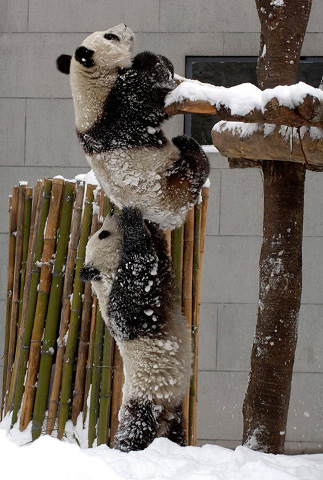
\includegraphics{panda-giving-another-panda-a-hand-sm.jpg}
\end{figure}

    \subsection{Pandas}\label{pandas}

\begin{itemize}
\itemsep1pt\parskip0pt\parsep0pt
\item
  Tabular, Timeseries, Matrix Data - labeled or not
\item
  Sensible handling of missing data and data alignment
\item
  Data selection, slicing and reshaping features
\item
  Robust data import utilities.
\item
  Advanced time series capabilities
\end{itemize}

    \subsection{Data Structures}\label{data-structures}

\begin{itemize}
\itemsep1pt\parskip0pt\parsep0pt
\item
  Series - 1D labeled array
\item
  DataFrame - 2D labeled array
\item
  Panel - 3D labeled array (More D)
\end{itemize}

    \section{Assumed Imports}\label{assumed-imports}

In my code samples, assume I import the following

    \begin{Verbatim}[commandchars=\\\{\}]
{\color{incolor}In [{\color{incolor}5}]:} \PY{k+kn}{import} \PY{n+nn}{pandas} \PY{k+kn}{as} \PY{n+nn}{pd}
        \PY{k+kn}{import} \PY{n+nn}{numpy} \PY{k+kn}{as} \PY{n+nn}{np}
\end{Verbatim}

    \section{Series}\label{series}

\begin{itemize}
\itemsep1pt\parskip0pt\parsep0pt
\item
  one-dimensional labeled array
\item
  holds any data type
\item
  axis labels known as index
\item
  implicit integert indexes
\item
  \texttt{dict}-like
\end{itemize}

    \section{Create a Simple Series}\label{create-a-simple-series}

    \begin{Verbatim}[commandchars=\\\{\}]
{\color{incolor}In [{\color{incolor}6}]:} \PY{n}{s1} \PY{o}{=} \PY{n}{pd}\PY{o}{.}\PY{n}{Series}\PY{p}{(}\PY{p}{[}\PY{l+m+mi}{1}\PY{p}{,} \PY{l+m+mi}{2}\PY{p}{,} \PY{l+m+mi}{3}\PY{p}{,} \PY{l+m+mi}{4}\PY{p}{,} \PY{l+m+mi}{5}\PY{p}{]}\PY{p}{)}
        \PY{n}{s1}
\end{Verbatim}

            \begin{Verbatim}[commandchars=\\\{\}]
{\color{outcolor}Out[{\color{outcolor}6}]:} 0    1
        1    2
        2    3
        3    4
        4    5
        dtype: int64
\end{Verbatim}
        
    \section{Series Operations}\label{series-operations}

    \begin{Verbatim}[commandchars=\\\{\}]
{\color{incolor}In [{\color{incolor}7}]:} \PY{c}{\PYZsh{} integer multiplication}
        \PY{k}{print} \PY{n}{s1} \PY{o}{*} \PY{l+m+mi}{5}
\end{Verbatim}

    \begin{Verbatim}[commandchars=\\\{\}]
0     5
1    10
2    15
3    20
4    25
dtype: int64
    \end{Verbatim}

    \section{Series Operations - Cont.}\label{series-operations---cont.}

    \begin{Verbatim}[commandchars=\\\{\}]
{\color{incolor}In [{\color{incolor}8}]:} \PY{c}{\PYZsh{} float multiplication}
        \PY{k}{print} \PY{n}{s1} \PY{o}{*} \PY{l+m+mf}{5.0}
\end{Verbatim}

    \begin{Verbatim}[commandchars=\\\{\}]
0     5
1    10
2    15
3    20
4    25
dtype: float64
    \end{Verbatim}

    \section{Series Index}\label{series-index}

    \begin{Verbatim}[commandchars=\\\{\}]
{\color{incolor}In [{\color{incolor}9}]:} \PY{n}{s2} \PY{o}{=} \PY{n}{pd}\PY{o}{.}\PY{n}{Series}\PY{p}{(}\PY{p}{[}\PY{l+m+mi}{1}\PY{p}{,} \PY{l+m+mi}{2}\PY{p}{,} \PY{l+m+mi}{3}\PY{p}{,} \PY{l+m+mi}{4}\PY{p}{,} \PY{l+m+mi}{5}\PY{p}{]}\PY{p}{,}
                       \PY{n}{index}\PY{o}{=}\PY{p}{[}\PY{l+s}{\PYZsq{}}\PY{l+s}{a}\PY{l+s}{\PYZsq{}}\PY{p}{,} \PY{l+s}{\PYZsq{}}\PY{l+s}{b}\PY{l+s}{\PYZsq{}}\PY{p}{,} \PY{l+s}{\PYZsq{}}\PY{l+s}{c}\PY{l+s}{\PYZsq{}}\PY{p}{,} \PY{l+s}{\PYZsq{}}\PY{l+s}{d}\PY{l+s}{\PYZsq{}}\PY{p}{,} \PY{l+s}{\PYZsq{}}\PY{l+s}{e}\PY{l+s}{\PYZsq{}}\PY{p}{]}\PY{p}{)}
        \PY{n}{s2}
\end{Verbatim}

            \begin{Verbatim}[commandchars=\\\{\}]
{\color{outcolor}Out[{\color{outcolor}9}]:} a    1
        b    2
        c    3
        d    4
        e    5
        dtype: int64
\end{Verbatim}
        
    \section{Date Convenience Functions}\label{date-convenience-functions}

A quick aside \ldots{}

    \begin{Verbatim}[commandchars=\\\{\}]
{\color{incolor}In [{\color{incolor}10}]:} \PY{n}{dates} \PY{o}{=} \PY{n}{pd}\PY{o}{.}\PY{n}{date\PYZus{}range}\PY{p}{(}\PY{l+s}{\PYZsq{}}\PY{l+s}{20130626}\PY{l+s}{\PYZsq{}}\PY{p}{,} \PY{n}{periods}\PY{o}{=}\PY{l+m+mi}{5}\PY{p}{)}
         \PY{k}{print} \PY{n}{dates}
         \PY{k}{print}
         \PY{k}{print} \PY{n}{dates}\PY{p}{[}\PY{l+m+mi}{0}\PY{p}{]}
\end{Verbatim}

    \begin{Verbatim}[commandchars=\\\{\}]
<class 'pandas.tseries.index.DatetimeIndex'>
[2013-06-26, \ldots, 2013-06-30]
Length: 5, Freq: D, Timezone: None

2013-06-26 00:00:00
    \end{Verbatim}

    \section{Datestamps as Index}\label{datestamps-as-index}

    \begin{Verbatim}[commandchars=\\\{\}]
{\color{incolor}In [{\color{incolor}11}]:} \PY{n}{s3} \PY{o}{=} \PY{n}{pd}\PY{o}{.}\PY{n}{Series}\PY{p}{(}\PY{p}{[}\PY{l+m+mi}{1}\PY{p}{,} \PY{l+m+mi}{2}\PY{p}{,} \PY{l+m+mi}{3}\PY{p}{,} \PY{l+m+mi}{4}\PY{p}{,} \PY{l+m+mi}{5}\PY{p}{]}\PY{p}{,} \PY{n}{index}\PY{o}{=}\PY{n}{dates}\PY{p}{)}
         \PY{k}{print} \PY{n}{s3}
\end{Verbatim}

    \begin{Verbatim}[commandchars=\\\{\}]
2013-06-26    1
2013-06-27    2
2013-06-28    3
2013-06-29    4
2013-06-30    5
Freq: D, dtype: int64
    \end{Verbatim}

    \section{Selecting By Index}\label{selecting-by-index}

Note that the integer index is retained along with the new date index.

    \begin{Verbatim}[commandchars=\\\{\}]
{\color{incolor}In [{\color{incolor}12}]:} \PY{k}{print} \PY{n}{s3}\PY{p}{[}\PY{l+m+mi}{0}\PY{p}{]}
         \PY{k}{print} \PY{n+nb}{type}\PY{p}{(}\PY{n}{s3}\PY{p}{[}\PY{l+m+mi}{0}\PY{p}{]}\PY{p}{)}
         \PY{k}{print}
         \PY{k}{print} \PY{n}{s3}\PY{p}{[}\PY{l+m+mi}{1}\PY{p}{:}\PY{l+m+mi}{3}\PY{p}{]}
         \PY{k}{print} \PY{n+nb}{type}\PY{p}{(}\PY{n}{s3}\PY{p}{[}\PY{l+m+mi}{1}\PY{p}{:}\PY{l+m+mi}{3}\PY{p}{]}\PY{p}{)}
\end{Verbatim}

    \begin{Verbatim}[commandchars=\\\{\}]
1
<type 'numpy.int64'>

2013-06-27    2
2013-06-28    3
Freq: D, dtype: int64
<class 'pandas.core.series.Series'>
    \end{Verbatim}

    \section{Selecting by value}\label{selecting-by-value}

    \begin{Verbatim}[commandchars=\\\{\}]
{\color{incolor}In [{\color{incolor}13}]:} \PY{n}{s3}\PY{p}{[}\PY{n}{s3} \PY{o}{\PYZlt{}} \PY{l+m+mi}{3}\PY{p}{]}
\end{Verbatim}

            \begin{Verbatim}[commandchars=\\\{\}]
{\color{outcolor}Out[{\color{outcolor}13}]:} 2013-06-26    1
         2013-06-27    2
         Freq: D, dtype: int64
\end{Verbatim}
        
    \section{Selecting by Label (Date)}\label{selecting-by-label-date}

    \begin{Verbatim}[commandchars=\\\{\}]
{\color{incolor}In [{\color{incolor}14}]:} \PY{n}{s3}\PY{p}{[}\PY{l+s}{\PYZsq{}}\PY{l+s}{20130626}\PY{l+s}{\PYZsq{}}\PY{p}{:}\PY{l+s}{\PYZsq{}}\PY{l+s}{20130628}\PY{l+s}{\PYZsq{}}\PY{p}{]}
\end{Verbatim}

            \begin{Verbatim}[commandchars=\\\{\}]
{\color{outcolor}Out[{\color{outcolor}14}]:} 2013-06-26    1
         2013-06-27    2
         2013-06-28    3
         Freq: D, dtype: int64
\end{Verbatim}
        
    \subsection{Series Wrapup}\label{series-wrapup}

Things not covered but you should look into:

\begin{itemize}
\item
  Other instantiation options: \texttt{dict}
\item
  Operator Handling of missing data \texttt{NaN}
\item
  Reforming Data and Indexes
\item
  Boolean Indexing
\item
  Other Series Attributes:
\item
  \texttt{index} - \texttt{index.name}
\item
  \texttt{name} - Series name
\end{itemize}

    \subsection{DataFrame}\label{dataframe}

\begin{itemize}
\itemsep1pt\parskip0pt\parsep0pt
\item
  2-dimensional labeled data structure
\item
  Like a SQL Table, Spreadsheet or \texttt{dict} of \texttt{Series}
  objects.
\item
  Columns of potentially different types
\item
  Operations, slicing and other behavior just like \texttt{Series}
\end{itemize}

    \section{DataFrame - Simple}\label{dataframe---simple}

    \begin{Verbatim}[commandchars=\\\{\}]
{\color{incolor}In [{\color{incolor}15}]:} \PY{n}{data1} \PY{o}{=} \PY{n}{pd}\PY{o}{.}\PY{n}{DataFrame}\PY{p}{(}\PY{n}{np}\PY{o}{.}\PY{n}{random}\PY{o}{.}\PY{n}{rand}\PY{p}{(}\PY{l+m+mi}{4}\PY{p}{,} \PY{l+m+mi}{4}\PY{p}{)}\PY{p}{)}
         \PY{n}{data1}
\end{Verbatim}

            \begin{Verbatim}[commandchars=\\\{\}]
{\color{outcolor}Out[{\color{outcolor}15}]:}           0         1         2         3
         0  0.371333  0.788792  0.869380  0.084323
         1  0.490858  0.134202  0.816307  0.019157
         2  0.839547  0.721638  0.544628  0.042547
         3  0.098594  0.954038  0.306561  0.689759
\end{Verbatim}
        
    \section{DataFrame - Index/Column
Names}\label{dataframe---indexcolumn-names}

    \begin{Verbatim}[commandchars=\\\{\}]
{\color{incolor}In [{\color{incolor}16}]:} \PY{n}{dates} \PY{o}{=} \PY{n}{pd}\PY{o}{.}\PY{n}{date\PYZus{}range}\PY{p}{(}\PY{l+s}{\PYZsq{}}\PY{l+s}{20130626}\PY{l+s}{\PYZsq{}}\PY{p}{,} \PY{n}{periods}\PY{o}{=}\PY{l+m+mi}{4}\PY{p}{)}
         \PY{n}{data2} \PY{o}{=} \PY{n}{pd}\PY{o}{.}\PY{n}{DataFrame}\PY{p}{(}
             \PY{n}{np}\PY{o}{.}\PY{n}{random}\PY{o}{.}\PY{n}{rand}\PY{p}{(}\PY{l+m+mi}{4}\PY{p}{,} \PY{l+m+mi}{4}\PY{p}{)}\PY{p}{,}
             \PY{n}{index}\PY{o}{=}\PY{n}{dates}\PY{p}{,} \PY{n}{columns}\PY{o}{=}\PY{n+nb}{list}\PY{p}{(}\PY{l+s}{\PYZsq{}}\PY{l+s}{ABCD}\PY{l+s}{\PYZsq{}}\PY{p}{)}\PY{p}{)}
         \PY{n}{data2}
\end{Verbatim}

            \begin{Verbatim}[commandchars=\\\{\}]
{\color{outcolor}Out[{\color{outcolor}16}]:}                    A         B         C         D
         2013-06-26  0.572954  0.785437  0.089758  0.872083
         2013-06-27  0.857868  0.779294  0.453022  0.836332
         2013-06-28  0.715369  0.355922  0.750194  0.770045
         2013-06-29  0.409056  0.452993  0.937368  0.118998
\end{Verbatim}
        
    \section{DataFrame - Operations}\label{dataframe---operations}

    \begin{Verbatim}[commandchars=\\\{\}]
{\color{incolor}In [{\color{incolor}17}]:} \PY{n}{data2}\PY{p}{[}\PY{l+s}{\PYZsq{}}\PY{l+s}{E}\PY{l+s}{\PYZsq{}}\PY{p}{]} \PY{o}{=} \PY{n}{data2}\PY{p}{[}\PY{l+s}{\PYZsq{}}\PY{l+s}{B}\PY{l+s}{\PYZsq{}}\PY{p}{]} \PY{o}{+} \PY{l+m+mi}{5} \PY{o}{*} \PY{n}{data2}\PY{p}{[}\PY{l+s}{\PYZsq{}}\PY{l+s}{C}\PY{l+s}{\PYZsq{}}\PY{p}{]}
         \PY{n}{data2}
\end{Verbatim}

            \begin{Verbatim}[commandchars=\\\{\}]
{\color{outcolor}Out[{\color{outcolor}17}]:}                    A         B         C         D         E
         2013-06-26  0.572954  0.785437  0.089758  0.872083  1.234225
         2013-06-27  0.857868  0.779294  0.453022  0.836332  3.044402
         2013-06-28  0.715369  0.355922  0.750194  0.770045  4.106891
         2013-06-29  0.409056  0.452993  0.937368  0.118998  5.139832
\end{Verbatim}
        
    See? You never need Excel again!

    \section{DataFrame - Column Access}\label{dataframe---column-access}

Deleting a column.

    \begin{Verbatim}[commandchars=\\\{\}]
{\color{incolor}In [{\color{incolor}18}]:} \PY{c}{\PYZsh{} Deleting a Column}
         \PY{k}{del} \PY{n}{data2}\PY{p}{[}\PY{l+s}{\PYZsq{}}\PY{l+s}{E}\PY{l+s}{\PYZsq{}}\PY{p}{]}
         \PY{n}{data2}
\end{Verbatim}

            \begin{Verbatim}[commandchars=\\\{\}]
{\color{outcolor}Out[{\color{outcolor}18}]:}                    A         B         C         D
         2013-06-26  0.572954  0.785437  0.089758  0.872083
         2013-06-27  0.857868  0.779294  0.453022  0.836332
         2013-06-28  0.715369  0.355922  0.750194  0.770045
         2013-06-29  0.409056  0.452993  0.937368  0.118998
\end{Verbatim}
        
    \section{DataFrame}\label{dataframe}

Remember this, data2, for the next examples.

    \begin{Verbatim}[commandchars=\\\{\}]
{\color{incolor}In [{\color{incolor}19}]:} \PY{n}{data2}
\end{Verbatim}

            \begin{Verbatim}[commandchars=\\\{\}]
{\color{outcolor}Out[{\color{outcolor}19}]:}                    A         B         C         D
         2013-06-26  0.572954  0.785437  0.089758  0.872083
         2013-06-27  0.857868  0.779294  0.453022  0.836332
         2013-06-28  0.715369  0.355922  0.750194  0.770045
         2013-06-29  0.409056  0.452993  0.937368  0.118998
\end{Verbatim}
        
    \section{DataFrame - Column Access}\label{dataframe---column-access}

As a dict

    \begin{Verbatim}[commandchars=\\\{\}]
{\color{incolor}In [{\color{incolor}20}]:} \PY{n}{data2}\PY{p}{[}\PY{l+s}{\PYZsq{}}\PY{l+s}{B}\PY{l+s}{\PYZsq{}}\PY{p}{]}
\end{Verbatim}

            \begin{Verbatim}[commandchars=\\\{\}]
{\color{outcolor}Out[{\color{outcolor}20}]:} 2013-06-26    0.785437
         2013-06-27    0.779294
         2013-06-28    0.355922
         2013-06-29    0.452993
         Freq: D, Name: B, dtype: float64
\end{Verbatim}
        
    \section{DataFrame - Column Access}\label{dataframe---column-access}

As an attribute

    \begin{Verbatim}[commandchars=\\\{\}]
{\color{incolor}In [{\color{incolor}21}]:} \PY{n}{data2}\PY{o}{.}\PY{n}{B}
\end{Verbatim}

            \begin{Verbatim}[commandchars=\\\{\}]
{\color{outcolor}Out[{\color{outcolor}21}]:} 2013-06-26    0.785437
         2013-06-27    0.779294
         2013-06-28    0.355922
         2013-06-29    0.452993
         Freq: D, Name: B, dtype: float64
\end{Verbatim}
        
    \section{DataFrame - Row Access}\label{dataframe---row-access}

By row label

    \begin{Verbatim}[commandchars=\\\{\}]
{\color{incolor}In [{\color{incolor}22}]:} \PY{n}{data2}\PY{o}{.}\PY{n}{loc}\PY{p}{[}\PY{l+s}{\PYZsq{}}\PY{l+s}{20130627}\PY{l+s}{\PYZsq{}}\PY{p}{]}    
\end{Verbatim}

            \begin{Verbatim}[commandchars=\\\{\}]
{\color{outcolor}Out[{\color{outcolor}22}]:} A    0.857868
         B    0.779294
         C    0.453022
         D    0.836332
         Name: 2013-06-27 00:00:00, dtype: float64
\end{Verbatim}
        
    \section{DataFrame - Row Access}\label{dataframe---row-access}

By integer location

    \begin{Verbatim}[commandchars=\\\{\}]
{\color{incolor}In [{\color{incolor}23}]:} \PY{n}{data2}\PY{o}{.}\PY{n}{iloc}\PY{p}{[}\PY{l+m+mi}{1}\PY{p}{]}
\end{Verbatim}

            \begin{Verbatim}[commandchars=\\\{\}]
{\color{outcolor}Out[{\color{outcolor}23}]:} A    0.857868
         B    0.779294
         C    0.453022
         D    0.836332
         Name: 2013-06-27 00:00:00, dtype: float64
\end{Verbatim}
        
    \section{DataFrame - Cell Access}\label{dataframe---cell-access}

Access column, then row or use iloc and row/column indexes.

    \begin{Verbatim}[commandchars=\\\{\}]
{\color{incolor}In [{\color{incolor}24}]:} \PY{k}{print} \PY{n}{data2}\PY{o}{.}\PY{n}{B}\PY{p}{[}\PY{l+m+mi}{0}\PY{p}{]}
         \PY{k}{print} \PY{n}{data2}\PY{p}{[}\PY{l+s}{\PYZsq{}}\PY{l+s}{B}\PY{l+s}{\PYZsq{}}\PY{p}{]}\PY{p}{[}\PY{l+m+mi}{0}\PY{p}{]}
         \PY{k}{print} \PY{n}{data2}\PY{o}{.}\PY{n}{iloc}\PY{p}{[}\PY{l+m+mi}{0}\PY{p}{,}\PY{l+m+mi}{1}\PY{p}{]}  \PY{c}{\PYZsh{} [row,column] }
\end{Verbatim}

    \begin{Verbatim}[commandchars=\\\{\}]
0.785436968548
0.785436968548
0.785436968548
    \end{Verbatim}

    \section{DataFrame - Taking a Peek}\label{dataframe---taking-a-peek}

Look at the beginning of the DataFrame

    \begin{Verbatim}[commandchars=\\\{\}]
{\color{incolor}In [{\color{incolor}25}]:} \PY{n}{data3} \PY{o}{=} \PY{n}{pd}\PY{o}{.}\PY{n}{DataFrame}\PY{p}{(}\PY{n}{np}\PY{o}{.}\PY{n}{random}\PY{o}{.}\PY{n}{rand}\PY{p}{(}\PY{l+m+mi}{100}\PY{p}{,} \PY{l+m+mi}{4}\PY{p}{)}\PY{p}{)}
         \PY{n}{data3}\PY{o}{.}\PY{n}{head}\PY{p}{(}\PY{p}{)}
\end{Verbatim}

            \begin{Verbatim}[commandchars=\\\{\}]
{\color{outcolor}Out[{\color{outcolor}25}]:}           0         1         2         3
         0  0.127258  0.981462  0.820096  0.650613
         1  0.471623  0.118745  0.595012  0.205356
         2  0.802777  0.398816  0.383789  0.025648
         3  0.368724  0.922648  0.850099  0.659503
         4  0.889618  0.565936  0.056413  0.768219
\end{Verbatim}
        
    \section{DataFrame - Taking a Peek}\label{dataframe---taking-a-peek}

Look at the end of the DataFrame.

    \begin{Verbatim}[commandchars=\\\{\}]
{\color{incolor}In [{\color{incolor}26}]:} \PY{n}{data3}\PY{o}{.}\PY{n}{tail}\PY{p}{(}\PY{p}{)}
\end{Verbatim}

            \begin{Verbatim}[commandchars=\\\{\}]
{\color{outcolor}Out[{\color{outcolor}26}]:}            0         1         2         3
         95  0.332815  0.920505  0.808580  0.161875
         96  0.348941  0.532944  0.921147  0.736528
         97  0.305776  0.747903  0.161359  0.808279
         98  0.141267  0.878946  0.537137  0.157560
         99  0.862024  0.519265  0.172454  0.665810
\end{Verbatim}
        
    \section{DataFrame Wrap Up}\label{dataframe-wrap-up}

Just remember,

\begin{itemize}
\itemsep1pt\parskip0pt\parsep0pt
\item
  A \texttt{DataFrame} is just a bunch of \texttt{Series} grouped
  together.
\item
  Any one dimensional slice returns a \texttt{Series}
\item
  Any two dimensional slice returns another \texttt{DataFrame}.
\item
  Elements are typically NumPy types or Objects.
\end{itemize}

    \section{Panel}\label{panel}

Like DataFrame but 3 or more dimensions.

    \section{IO Tools}\label{io-tools}

Robust IO tools to read in data from a variety of sources

\begin{itemize}
\itemsep1pt\parskip0pt\parsep0pt
\item
  CSV -
  \href{http://pandas.pydata.org/pandas-docs/stable/io.html\#io-read-csv-table}{pd.read\_csv()}
\item
  Clipboard -
  \href{http://pandas.pydata.org/pandas-docs/stable/io.html\#clipboard}{pd.read\_clipboard()}
\item
  SQL -
  \href{http://pandas.pydata.org/pandas-docs/stable/io.html\#sql-queries}{pd.read\_sql\_table()}
\item
  Excel -
  \href{http://pandas.pydata.org/pandas-docs/stable/io.html\#io-excel}{pd.read\_excel()}
\end{itemize}

    \section{Plotting}\label{plotting}

\begin{itemize}
\itemsep1pt\parskip0pt\parsep0pt
\item
  Matplotlib -
  \href{http://pandas.pydata.org/pandas-docs/stable/visualization.html\#plotting-with-matplotlib}{s.plot()}
  - Standard Python Plotting Library
\item
  Trellis -
  \href{http://pandas.pydata.org/pandas-docs/stable/rplot.html}{rplot()}
  - An `R' inspired Matplotlib based plotting tool
\end{itemize}

    \section{Bringing it Together - Data}\label{bringing-it-together---data}

The csv file (\texttt{phx-temps.csv}) contains Phoenix weather data from
GSOD::

\begin{verbatim}
1973-01-01 00:00:00,53.1,37.9
1973-01-02 00:00:00,57.9,37.0
...
2012-12-30 00:00:00,64.9,39.0
2012-12-31 00:00:00,55.9,41.0
\end{verbatim}

    \section{Bringing it Together - Code}\label{bringing-it-together---code}

Simple \texttt{read\_csv()}

    \begin{Verbatim}[commandchars=\\\{\}]
{\color{incolor}In [{\color{incolor}27}]:} \PY{c}{\PYZsh{} simple readcsv}
         \PY{n}{phxtemps1} \PY{o}{=} \PY{n}{pd}\PY{o}{.}\PY{n}{read\PYZus{}csv}\PY{p}{(}\PY{l+s}{\PYZsq{}}\PY{l+s}{phx\PYZhy{}temps.csv}\PY{l+s}{\PYZsq{}}\PY{p}{)}
         \PY{n}{phxtemps1}\PY{o}{.}\PY{n}{head}\PY{p}{(}\PY{p}{)}
\end{Verbatim}

            \begin{Verbatim}[commandchars=\\\{\}]
{\color{outcolor}Out[{\color{outcolor}27}]:}    1973-01-01 00:00:00  53.1  37.9
         0  1973-01-02 00:00:00  57.9  37.0
         1  1973-01-03 00:00:00  59.0  37.0
         2  1973-01-04 00:00:00  57.9  41.0
         3  1973-01-05 00:00:00  54.0  39.9
         4  1973-01-06 00:00:00  55.9  37.9
\end{Verbatim}
        
    \section{Bringing it Together - Code}\label{bringing-it-together---code}

Advanced \texttt{read\_csv()}, parsing the dates and using them as the
index, and naming the columns.

    \begin{Verbatim}[commandchars=\\\{\}]
{\color{incolor}In [{\color{incolor}28}]:} \PY{c}{\PYZsh{} define index, parse dates, name columns}
         \PY{n}{phxtemps2} \PY{o}{=} \PY{n}{pd}\PY{o}{.}\PY{n}{read\PYZus{}csv}\PY{p}{(}
             \PY{l+s}{\PYZsq{}}\PY{l+s}{phx\PYZhy{}temps.csv}\PY{l+s}{\PYZsq{}}\PY{p}{,} \PY{n}{index\PYZus{}col}\PY{o}{=}\PY{l+m+mi}{0}\PY{p}{,}
             \PY{n}{names}\PY{o}{=}\PY{p}{[}\PY{l+s}{\PYZsq{}}\PY{l+s}{highs}\PY{l+s}{\PYZsq{}}\PY{p}{,} \PY{l+s}{\PYZsq{}}\PY{l+s}{lows}\PY{l+s}{\PYZsq{}}\PY{p}{]}\PY{p}{,} \PY{n}{parse\PYZus{}dates}\PY{o}{=}\PY{n+nb+bp}{True}\PY{p}{)}
         \PY{n}{phxtemps2}\PY{o}{.}\PY{n}{head}\PY{p}{(}\PY{p}{)}
\end{Verbatim}

            \begin{Verbatim}[commandchars=\\\{\}]
{\color{outcolor}Out[{\color{outcolor}28}]:}             highs  lows
         1973-01-01   53.1  37.9
         1973-01-02   57.9  37.0
         1973-01-03   59.0  37.0
         1973-01-04   57.9  41.0
         1973-01-05   54.0  39.9
\end{Verbatim}
        
    \section{Bringing it Together - Plot}\label{bringing-it-together---plot}

    \begin{Verbatim}[commandchars=\\\{\}]
{\color{incolor}In [{\color{incolor}29}]:} \PY{k+kn}{import} \PY{n+nn}{matplotlib.pyplot} \PY{k+kn}{as} \PY{n+nn}{plt}
         \PY{o}{\PYZpc{}}\PY{k}{matplotlib} \PY{n}{inline} 
         \PY{n}{phxtemps2}\PY{o}{.}\PY{n}{plot}\PY{p}{(}\PY{p}{)}  \PY{c}{\PYZsh{} pandas convenience method}
\end{Verbatim}

            \begin{Verbatim}[commandchars=\\\{\}]
{\color{outcolor}Out[{\color{outcolor}29}]:} <matplotlib.axes.AxesSubplot at 0x7f9916ef4d90>
\end{Verbatim}
        
    \begin{center}
    \adjustimage{max size={0.9\linewidth}{0.9\paperheight}}{Pandas_and_Friends_files/Pandas_and_Friends_81_1.png}
    \end{center}
    { \hspace*{\fill} \\}
    
    Boo, Pandas and Friends would cry if they saw such a plot.

    \section{Bringing it Together - Plot}\label{bringing-it-together---plot}

Lets see a smaller slice of time:

    \begin{Verbatim}[commandchars=\\\{\}]
{\color{incolor}In [{\color{incolor}30}]:} \PY{n}{phxtemps2}\PY{p}{[}\PY{l+s}{\PYZsq{}}\PY{l+s}{20120101}\PY{l+s}{\PYZsq{}}\PY{p}{:}\PY{l+s}{\PYZsq{}}\PY{l+s}{20121231}\PY{l+s}{\PYZsq{}}\PY{p}{]}\PY{o}{.}\PY{n}{plot}\PY{p}{(}\PY{p}{)}
\end{Verbatim}

            \begin{Verbatim}[commandchars=\\\{\}]
{\color{outcolor}Out[{\color{outcolor}30}]:} <matplotlib.axes.AxesSubplot at 0x7f9916ae8290>
\end{Verbatim}
        
    \begin{center}
    \adjustimage{max size={0.9\linewidth}{0.9\paperheight}}{Pandas_and_Friends_files/Pandas_and_Friends_84_1.png}
    \end{center}
    { \hspace*{\fill} \\}
    
    \section{Bringing it Together - Plot}\label{bringing-it-together---plot}

Lets operate on the \texttt{DataFrame} \ldots{} lets take the differnce
between the highs and lows.

    \begin{Verbatim}[commandchars=\\\{\}]
{\color{incolor}In [{\color{incolor}31}]:} \PY{n}{phxtemps2}\PY{p}{[}\PY{l+s}{\PYZsq{}}\PY{l+s}{diff}\PY{l+s}{\PYZsq{}}\PY{p}{]} \PY{o}{=} \PY{n}{phxtemps2}\PY{o}{.}\PY{n}{highs} \PY{o}{\PYZhy{}} \PY{n}{phxtemps2}\PY{o}{.}\PY{n}{lows}
         \PY{n}{phxtemps2}\PY{p}{[}\PY{l+s}{\PYZsq{}}\PY{l+s}{20120101}\PY{l+s}{\PYZsq{}}\PY{p}{:}\PY{l+s}{\PYZsq{}}\PY{l+s}{20121231}\PY{l+s}{\PYZsq{}}\PY{p}{]}\PY{o}{.}\PY{n}{plot}\PY{p}{(}\PY{p}{)}
\end{Verbatim}

            \begin{Verbatim}[commandchars=\\\{\}]
{\color{outcolor}Out[{\color{outcolor}31}]:} <matplotlib.axes.AxesSubplot at 0x7f99168bec10>
\end{Verbatim}
        
    \begin{center}
    \adjustimage{max size={0.9\linewidth}{0.9\paperheight}}{Pandas_and_Friends_files/Pandas_and_Friends_86_1.png}
    \end{center}
    { \hspace*{\fill} \\}
    
    \section{Pandas Alternatives}\label{pandas-alternatives}

\begin{itemize}
\itemsep1pt\parskip0pt\parsep0pt
\item
  AstroPy seems to have similar data structures.
\item
  I suspect there are others.
\end{itemize}

    \subsection{References}\label{references}

\begin{itemize}
\itemsep1pt\parskip0pt\parsep0pt
\item
  \href{http://pandas.pydata.org/pandas-docs/stable/index.html}{Pandas
  Documentation}
\item
  \href{http://www.amazon.com/Python-Data-Analysis-Wes-McKinney/dp/1449319793/}{Python
  for Data Analysis}
\item
  \href{https://github.com/desertpy/presentations}{Presentation Source}
\end{itemize}

    \section{Thanks! - Pandas and
Friends}\label{thanks---pandas-and-friends}

\begin{itemize}
\itemsep1pt\parskip0pt\parsep0pt
\item
  Austin Godber
\item
  Mail: godber@uberhip.com
\item
  Twitter: @godber
\item
  Presented at \href{http://desertpy.com}{DesertPy}, Jan 2015.
\end{itemize}


    % Add a bibliography block to the postdoc
    
    
    
    \end{document}
